\xchapter{Ciclo de vida de software acadêmico de análise estática}{}
\label{estudo3}

Este capítulo apresenta
um estudo para caracterização do estágio de evolução de software acadêmico de análise estática.
Os estágios de evolução do software são os definidos pelo modelo 
{\it ``Staged Model for Software Evolution''} \cite{rajlich2000staged}
e as características do projeto de software acadêmico consideradas são 
número de lançamentos e
número de módulos no código fonte.

O estudo avaliou o ciclo de vida de software acadêmico coletando
dados do código fonte através de análise estática com o apoio da
ferramenta Analizo \cite{terceiro2010analizo}.
Esta análise revelou que a maior parte dos projetos
estão em estágio inicial de desenvolvimento ou encerrados.

A seção \ref{estudo3:introducao} contextualiza o estudo,
a seção \ref{estudo3:escopo} descreve o objetivo e apresenta as questões de pesquisa,
a seção \ref{estudo3:planejamento} apresenta um planejamento do estudo,
as seções \ref{estudo3:preparacao} e \ref{estudo3:coleta} apresentam detalhes sobre a preparação e execução da coleta de dados,
as seções \ref{estudo3:analise} e \ref{estudo3:interpretacao} apresentam a análise e interpretação dos dados e
a seção \ref{estudo3:conclusoes} traça as conclusões finais deste estudo.

\section{Motivação} \label{estudo3:introducao} % {{{

Segundo o {\it ``Staged Model for Software Evolution''} \cite{rajlich2000staged},
o ciclo de vida de um produto de software tem início no estágio
de evolução chamado {\it ``Initial development''}, no qual a primeira versão funcional
do software é desenvolvida. A partir daí, ao longo de sua vida,
o software em evolução pode passar pelos estágios de 
{\it``Evolution''}, {\it ``Servicing''}, {\it ``Phaseout''}, até o encerramento de seu ciclo
no estágio de {\it ``Closedown''}, quando as empresas detentoras do
software o retiram do mercado \cite{rajlich2000staged}.

Em modelos de produção distintos e não-tradicionais, como é o modelo de desenvolvimento de
software acadêmico ou o modelo de software livre, por exemplo, o ciclo de vida do software pode
variar. No modelo {\it ``Staged Model for Software Evolution''} adaptado a
projetos software livre \cite{capiluppi2007adapting}, por exemplo, o ciclo de
vida do software não se encerra na fase de {\it ``Closedown''}, uma vez que estes projetos
não são retirados do mercado por empresas, podendo haver um caminho de retorno
entre as diversas fases, incluindo o retorno para a fase {\it
``Initial development''}, por exemplo.

Os projetos de software acadêmico caracterizados neste estudo são considerados
como projetos de software livre sob a perspectiva do modelo proposto por
\citeonline{capiluppi2007adapting}; uma vez que não há entre eles projetos
comerciais de propriedade exclusiva de empresas, enquadram-se muito melhor
neste modelo do que no modelo tradicional de software comercial não-livre
originalmente proposto por \citeonline{rajlich2000staged}.

A caracterização de projetos de software acadêmico de análise estática quanto
ao ciclo de vida será feita sob a perspectiva de cientistas desenvolvedores e
usuários finais de software interessados em compreender em que estágio de
desenvolvimento e evolução estão os projetos do ecossistema de software
acadêmico de análise estática. Tal informação pode ser 
útil ao se tomar decisão de adotar um certo software acadêmico para uso ou mesmo como
objeto de contribuição (ver capítulo~\ref{estudo2}).

Neste estudo, \textit{módulo} refere-se \`{a}s unidades que compõem um sistema de software.  
Paradigmas e linguagens de programação possuem uma ou mais
construções que fazem o papel de módulo -- ``classes'', ``aspectos'', ``tipos
abstratos de dados'', ou ``arquivos-fonte'' -- com propriedades que poderão
servir para caracterização do software acadêmico.

% }}}

\section{Escopo} \label{estudo3:escopo} % {{{

Projetos de software acadêmico de análise estática publicados nas 
conferências ASE e SCAM 
são nosso principal objeto de estudo.
Queremos saber em qual estágio de evolução estão os projetos de software
acadêmico de análise estática publicados nas conferências ASE e SCAM.

O objetivo da pesquisa está definido segundo a estrutura GQM \cite{basili1994goal}.

\subsection{Definição do Objetivo}

\begin{description}

  \item{\bf Objeto de estudo.}
    O objeto de estudo são projetos de software acadêmico de análise estática
    publicados em artigos científicos e seu estágio de evolução no ciclo de
    vida de software, conforme definido na seção~\ref{estudo3:introducao}.

  \item{\bf Propósito.}
    O propósito do estudo é caracterizar em qual estágio de evolução
    encontra-se cada software acadêmico de análise estática. O estudo
    contribuirá para a análise da desordem disfuncional caótica no domínio de
    análise estática. 

  \item{\bf Perspectiva.}
    A perspectiva considerada é a do cientista desenvolvedor e usuário final, isto é, o pesquisador
    que deseja saber em que estágio de evolução estão os projetos de software acadêmico do domínio
    de interesse. A perspectiva a ser considerada também é a do pesquisador que deseja
    conhecer ferramentas de análise estática para uso em sua pesquisa.

  \item{\bf Foco de qualidade.}
    O principal foco de qualidade estudado é a modularidade do software
    acadêmico de análise estática, com ênfase nos aspectos de lançamentos e
    versões do projeto, especialmente sobre o tamanho do software em número de
    módulos.

  \item{\bf Contexto.}
    O estudo foi conduzido com projetos de software acadêmico de análise
    estática publicados nas conferências ASE e SCAM.

\end{description}

\subsection{Sumário da Definição}

Analisar os \textit{projetos de software acadêmico de análise estática} publicados
com o propósito de \textit{caracterizá-los}
com respeito ao seu \textit{estágio de evolução no ciclo de vida}
na perspectiva de \textit{cientistas usuários finais e desenvolvedores de software}
no contexto das \textit{conferências de Engenharia de Software ASE e SCAM}.

\subsection{Questões de Pesquisa}

Neste estudo as seguintes questões de pesquisa, a respeito dos projetos de
software acadêmico de análise estática publicados nas conferências ASE e SCAM,
e seu ciclo de vida serão investigadas:

\newcommand{\EstudoTresQuestaoUm}{
  Em qual estágio de evolução estão os projetos de software acadêmico de
  análise estática publicados nas conferências ASE e SCAM em relação ao seu
  ciclo de vida?
}

\begin{description}
  \item [Q1:] \EstudoTresQuestaoUm

    Queremos saber com esta questão quais projetos de software acadêmico de
    análise estática continuam evoluindo após a sua publicação e em que nível
    de evolução se encontram.
\end{description}

\subsection{Métricas}

Para responder às questões de pesquisas, as seguintes métricas serão usadas:

\begin{enumerate}
  \item Número de lançamentos de cada projeto com informações sobre versão e data
  \item Número de lançamentos com código fonte disponível para download
  \item Número de módulos no código fonte de cada lançamento/versão
\end{enumerate}

% }}}

\section{Planejamento do Estudo} \label{estudo3:planejamento} % {{{

Este estudo foi realizado a partir de uma análise preliminar dos dados existentes
de cada software, coletados previamente nos Capítulos \ref{estudo1} e
\ref{estudo2}. O objetivo de tal análise foi identificar quais projetos são candidatos a
terem mais dados coletados para compor a caracterização do seu ciclo de vida. 
Ao final do estudo, cada projeto será caracterizado em um dos estágios
de evolução apresentados na seção \ref{estudo3:introducao}.

Na análise preliminar deve-se identificar entre os projetos de software
acadêmico quais possuem disponibilidade de download, ou ao menos, presença
oficial online com informações do projeto sobre lançamentos, para coleta
dos seguintes dados:

\begin{itemize}
  \item Número da versão
  \item Data do lançamento
  \item URL para download do código fonte
\end{itemize}

As fontes para coleta de dados são o site do projeto, manuais, código fonte e
repositórios. Usualmente será utilizada mais de uma fonte para compor todas as
informações sobre os lançamentos de um certo software. Não é raro que os
projetos mudem a forma de lançamento, passando de um formato para outro, de uma
plataforma a outra, entre outras mudanças; essas informações devem ser
investigadas a fim de encontrar o máximo de informação possível.

Os projetos sem presença oficial online ou sem disponibilidade de download, ou
seja, com a URL indicada pelos seus autores originais indisponível,
não terão, consequentemente, informações sobre os lançamentos; dessa forma, estes
projetos serão caracterizados como software com ciclo de vida encerrado ({\it
Closedown}), uma vez que eles estão indisponíveis e inacessíveis a qualquer
potencial usuário interessado em utilizar o software.

Os demais projetos, aqueles com presença online, e com código fonte disponível,
tiveram o código fonte de cada lançamento copiado localmente para análise
estática e coleta da métrica representando o tamanho do software em número de
módulos. Foi feito o download do código fonte de cada versão e a ferramenta de
análise estática Analizo foi utilizada para extrair as informações do código
fonte.

Analizo é software livre, distribuído sob a licença GNU General Public License
versão 3. Seu código-fonte, bem como pacotes binários, manuais e tutoriais
podem ser obtidos em \url{http://www.analizo.org}. Analizo é escrito em Perl,
sua última versão 1.19.1 lançada em 01 de Setembro de 2016 foi a versão
utilizada neste estudo.

Apenas os projetos escritos nas linguagens de programação suportadas pelo Analizo 
-- C, C++ C\# e Java -- serão analisados.
O código fonte dos projetos escritos em
outras linguagens de programação não serão analisados; 
estes projetos serão caracterizados com base em informações disponíveis ou 
serão definidos como {\it Desconhecido} quando não for possível determinar 
o estágio de evolução com as informações disponíveis. Projetos com apenas um
lançamento serão considerados projetos em estágio inicial de desenvolvimento
({\it Initial development}).

% }}}

\section{Preparação} \label{estudo3:preparacao} % {{{

Seguindo o planejamento apresentado na seção \ref{estudo3:planejamento},
preparamos os arquivos e templates necessários para realizar a coleta e análise
dos dados, o conjunto de projetos de software acadêmico de análise estática e
os dados coletados nos Capítulos \ref{estudo1} e \ref{estudo2} serão também
utilizados aqui neste estudo.

\begin{lstlisting}[
caption={Arquivo releases.yml.},
label={releases-yml},
frame=single,
numbers=left
]
  source:
  versions:
    - version:
      source:
      released_at:
    - version:
      source:
      released_at:
\end{lstlisting}

Para cada projeto foi criado um arquivo \texttt{releases.yml} com a estrutura
apresentada na Listagem \ref{releases-yml}, nele serão registradas as
informações sobre os lançamentos de cada software. Os arquivos foram criados
manualmente, para os projetos sem informações sobre lançamentos o arquivo será
criado com um único campo indicando indisponibilidade com o seguinte conteúdo
\texttt{source: unavailable}.

Após criar os arquivos para a coleta de informações sobre os lançamentos,
implementamos um arquivo de template em
\texttt{templates/releases-table.tex.epl} para agregar os dados e apresentá-los
na seção \ref{estudo3:coleta}, Tabela \ref{releases-table}.

O Analizo e suas dependências foram instaladas, um script para automatizar a
execução da ferramenta {\it analizo metrics} para coletar o número de módulos
de cada lançamento foi desenvolvido. Este script, disponível em
\texttt{bin/run-analizo}, foi implementado em linguagem Perl e será apresentado
em mais detalhes no Apêndice \ref{reproducibilidade-do-estudo}.

As métricas serão agregadas no arquivo CSV \texttt{documents/metrics.csv}
gerado pelo template \texttt{templates/metrics.csv.epl}, este template consulta
os arquivos com os dados de cada lançamento criado pela execução do {\it analizo metrics}
e exibe, para cada projeto, todos os lançamentos e suas métricas.

Por fim, definimos uma estrutura para adicionar aos arquivos \texttt{software.yml} de
cada projeto a informação final sobre o atual estágio de evolução em relação ao
ciclo de vida do software, conforme mostra a Listagem \ref{software-yml-life-cycle}.

\begin{lstlisting}[
caption={Campos adicionados ao arquivo software.yml de cada projeto.},
label={software-yml-life-cycle},
frame=single,
numbers=left
]
  life_cycle:
    stage:
    review:
\end{lstlisting}

O campo \texttt{review} foi utilizado para registrar anotações em forma livre
sobre a análise dos dados, a avaliação de cada projeto é realizada
inspecionando manualmente os dados coletados, incluindo dados trazidos pelos
estudos anteriores, o campo \texttt{stage} contém o resultado final da
caracterização do ciclo de vida de cada software, este campo assumirá um dos
estágios de evolução conforme o modelo de evolução apresentado em
\ref{estudo3:introducao}.

% }}}

\section{Coleta de Dados} \label{estudo3:coleta} % {{{

Seguindo o planejamento e preparação descritos nas seções
\ref{estudo3:planejamento} e \ref{estudo3:preparacao}, iniciamos a coleta dos
dados, incluindo a coleta do número de lançamentos de cada projeto, informações
e código fonte de cada lançamento, bem como a métrica representando o número de
módulos do software em cada versão. Coletamos os dados sobre lançamentos,
fizemos o download do código fonte e executamos a ferramenta \texttt{analizo
metrics} para cada projeto, em cada versão.

Foi encontrado ao todo \ReleasesCount \ lançamentos, coletamos para cada
lançamento, quando disponível, número da versão, data de lançamento e URL para
download do código fonte. Destes lançamentos, \ReleasesAvailableCount \ possui
informação para download, 5 destes releases não tem código fonte, apenas
binários do software \texttt{s33}. Assim, deste total extraímos métricas
de código fonte de \ReleasesMetricsCount \ lançamentos.

Este total de métricas foi extraído de um conjunto de \ProjectsAnalizedCount \
projetos, os demais projetos não possuem código fonte disponível ou são
escritos em linguagem de programação não suportada pelo Analizo. Entre os anos
de \ReleasesYearFirst \ e \ReleasesYearLast.

Os lançamentos coletados do repositório, código fonte, sites, devem ser
organizados em ordem de data de lançamento, os mais antigos primeiros, numa
lista em ordem, sendo o último release o lançamento mais recente. Isto é
necessário uma vez que o número de versão de cada projeto não segue o mesmo
padrão, alterando de formatos entre releases distintos, a data de lançamento de
cada release também nem sempre está disponível, então a coleta deve garantir
que haja alguma ordem, então no momento da coleta deve-se avaliar a ordem dos
lançamentos e registrar no arquivo \texttt{releases.yml} na ordem correta.

% }}}

\section{Análise dos Dados} \label{estudo3:analise} % {{{

Analisamos as métricas e a variação em número de módulos entre as versões dos
projetos com lançamentos e código fonte disponível, analisamos também as
menções do tipo Uso e Contribuiçao para determinar se há atividade recente para
os projetos sem lançamentos atuais.

Iremos considerar projetos em fase de serviço ({\it Servicing}) aqueles que
apresentem variação pequena entre os lançamentos em relação ao tamanho do
projeto, em termos de número de módulos, abaixo de 10\% de variação ao longo
das versões será considerado {\it Servicing}, acima de 10\% está em evolução
({\it Evolution}), este número 10\% foi emprestado do trabalho de
\citeonline{capiluppi2007adapting}.

Cinco projetos não puderam ser caracterizados em relação ao estágio de
evolução, a Tabela \ref{releases-table} apreseta a caracterização final de
todos os projetos incluindo o número total de lançamentos e o período em que
estes lançamentos aconteceram.

\begin{longtable}{ l c c l | l c c l }
\caption{Número e período dos lançamentos de software acadêmico de análise estática.}
\label{releases-table} \\
  \hline
  \hhline{ l c c l | l c c l |}
  \endfirsthead
  \hhline{ l c c l | l c c l |}
  \hline
  \multirow{2}{*}{\textbf{ID}} & \multicolumn{2}{c}{\textbf{Lançamentos}} & \multirow{2}{*}{\textbf{Evolução}} & \multirow{2}{*}{\textbf{ID}} & \multicolumn{2}{c}{\textbf{Lançamentos}} & \multirow{2}{*}{\textbf{Evolução}} \\
           & \textbf{\#} & \textbf{Período} &                &            & \textbf{\#} & \textbf{Período} &  \\
  \hline
  \hhline{ l c c l | l c c l |}
  \endhead
  \hhline{----|----}
  \multicolumn{8}{c}{continua na próxima página} \\
  \hhline{----|----} \endfoot
  \hhline{----|----} \endlastfoot
  \multirow{2}{*}{\textbf{ID}} & \multicolumn{2}{c}{\textbf{Lançamentos}} & \multirow{2}{*}{\textbf{Evolução}} & \multirow{2}{*}{\textbf{ID}} & \multicolumn{2}{c}{\textbf{Lançamentos}} & \multirow{2}{*}{\textbf{Evolução}} \\
           & \textbf{\#} & \textbf{Período} &                &            & \textbf{\#} & \textbf{Período} &  \\
  \hline
      \texttt{s1} & 7 & 2015-2017 & Evolution &
        \texttt{s31} & - & - & Closedown  \\
      \texttt{s2} & 4 & 2010-2012 & Initial development &
        \texttt{s32} & 1 & 2006 & Desconhecido  \\
      \texttt{s3} & - & - & Closedown &
        \texttt{s33} & 5 & 2007-2010 & Desconhecido  \\
      \texttt{s4} & - & - & Closedown &
        \texttt{s34} & 1 & 2017 & Initial development  \\
      \texttt{s5} & - & - & Closedown &
        \texttt{s35} & 1 & 2017 & Initial development  \\
      \texttt{s6} & 36 & 2013-2017 & Servicing &
        \texttt{s36} & - & - & Closedown  \\
      \texttt{s7} & 7 & 2001-2004 & Initial development &
        \texttt{s37} & 5 & - & Initial development  \\
      \texttt{s8} & 4 & 2005 & Initial development &
        \texttt{s38} & - & - & Closedown  \\
      \texttt{s9} & - & - & Closedown &
        \texttt{s39} & - & - & Closedown  \\
      \texttt{s10} & 4 & - & Initial development &
        \texttt{s40} & 4 & 2011-2014 & Desconhecido  \\
      \texttt{s11} & - & - & Closedown &
        \texttt{s41} & - & - & Phaseout  \\
      \texttt{s12} & 2 & 2013-2014 & Initial development &
        \texttt{s42} & 1 & 2017 & Initial development  \\
      \texttt{s13} & - & - & Closedown &
        \texttt{s43} & 1 & 2008 & Initial development  \\
      \texttt{s14} & 1 & 2014 & Initial development &
        \texttt{s44} & - & - & Closedown  \\
      \texttt{s15} & - & - & Closedown &
        \texttt{s45} & - & - & Closedown  \\
      \texttt{s17} & 1 & 2014 & Initial development &
        \texttt{s46} & 5 & 2009-2010 & Initial development  \\
      \texttt{s16} & 1 & - & Initial development &
        \texttt{s47} & - & - & Closedown  \\
      \texttt{s18} & 25 & 2015-2017 & Servicing &
        \texttt{s48} & - & - & Closedown  \\
      \texttt{s19} & - & - & Closedown &
        \texttt{s49} & - & - & Closedown  \\
      \texttt{s20} & - & - & Closedown &
        \texttt{s50} & 6 & 2015-2017 & Evolution  \\
      \texttt{s21} & 1 & - & Initial development &
        \texttt{s51} & 18 & 2012-2016 & Servicing  \\
      \texttt{s22} & 1 & 2017 & Initial development &
        \texttt{s52} & 14 & 2011-2015 & Initial development  \\
      \texttt{s23} & - & - & Closedown &
        \texttt{s53} & - & - & Closedown  \\
      \texttt{s24} & 1 & - & Closedown &
        \texttt{s54} & 1 & - & Closedown  \\
      \texttt{s25} & 3 & 2013-2015 & Initial development &
        \texttt{s55} & 21 & 2010-2016 & Desconhecido  \\
      \texttt{s26} & 22 & 2013-2017 & Servicing &
        \texttt{s56} & - & - & Closedown  \\
      \texttt{s27} & 1 & - & Initial development &
        \texttt{s57} & - & - & Closedown  \\
      \texttt{s28} & 26 & 2013-2017 & Servicing &
        \texttt{s58} & 37 & 2006-2017 & Servicing  \\
      \texttt{s29} & 1 & 2013 & Initial development &
        \texttt{s59} & 34 & 2013-2015 & Desconhecido  \\
      \texttt{s30} & - & - & Closedown &
        \texttt{s60} & - & - & Closedown  \\
\end{longtable}


O projeto \texttt{s59} não foi caracterizado em relação ao estágio de evolução
apesar possuir muitas versões entre 2013 e 2015 por ser escrito em Erlang e
esta linguagem não ser suportada pelo Analizo. O mesmo ocorre com os projetos
\texttt{s55} escrito em Perl, e \texttt{s40} escrito em Rascal.  O projeto
\texttt{s33} disponível apenas em binários não possível ser analisado e o
projeto \texttt{s32} possui um histórico de lançamentos bastante confuso,
dificultando compreender quais pacotes fazem parte de qual versão ou
lançamento.

% }}}

\section{Interpretação dos Resultados} \label{estudo3:interpretacao} % {{{

\subsection{Q1 - \EstudoTresQuestaoUm}

Os \SoftwareCount \ projetos de software acadêmico de análise estática estão em
sua maioria em estágio inicial de desenvolvimento ou encerrados, representando
76\% de todos os projetos. Os demais 24\% dos projetos estão distribuídos entre
projetos em evolução, serviço, encerrando ou não puderam ser determinados,
conforme Figura \ref{life-cycle}.

\begin{figure}[h]
  \begin{minipage}{0.5\textwidth}
    \centering
    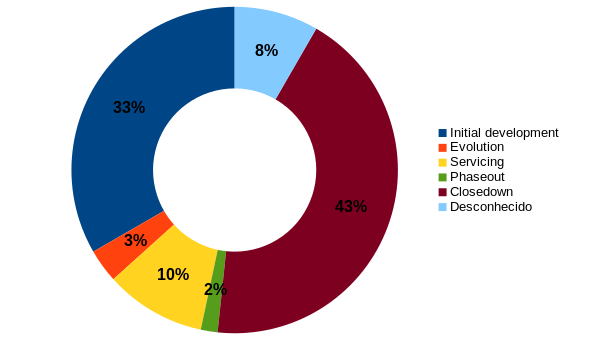
\includegraphics[scale=0.55]{imagens/life-cycle-pie.png}
  \end{minipage}
  \begin{minipage}{0.5\textwidth}
    \centering
    \begin{tabular}{l c}
  \hline
  {\bf Estágio} & {\bf Projetos} \\
  \hline
    Initial development & 20 \\
    Evolution & 2 \\
    Servicing & 6 \\
    Phaseout & 3 \\
    Closedown & 24 \\
    Desconhecido & 5 \\
  \hline
\end{tabular}

  \end{minipage}
  \caption{Número total de projetos identificados em cada estágio de evolução.}
  \label{life-cycle}
\end{figure}

Entre os projetos em fase de evolução ou serviço estão aqueles com maior número
de lançamentos. Os projetos em estágio {\it Initial development} possuem
características de ser software acadêmico do tipo Software Incidental ({\it
Incidental software}) e ter sido feito puramente para apoiar e facilitar
pesquisas, enquanto os projetos em estágio {\it Evolution} e {\it Servicing}
possi características de ser software acadêmico do tipo Prática de software
paralela ({\it A parallel software practice}) feito com objetivo de ser
utilizado por outros pesquisadores ou Um subcampo de software ({\it A Software
Sub-field}) onde o próprio software é considerado uma contribuição primária
para a Ciência.

\begin{figure}[h]
  \begin{minipage}{0.32\textwidth}
    \centering
    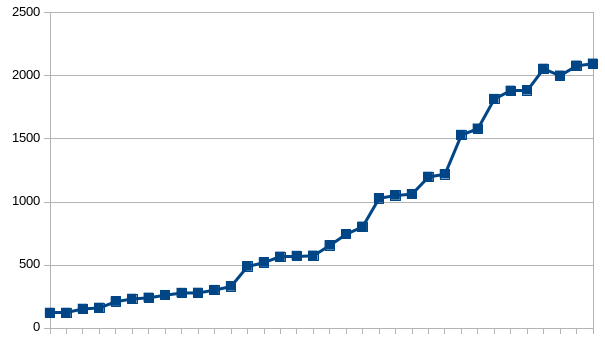
\includegraphics[scale=0.32]{imagens/evolution-s6.png}
    \texttt{s6}
  \end{minipage}
  \begin{minipage}{0.32\textwidth}
    \centering
    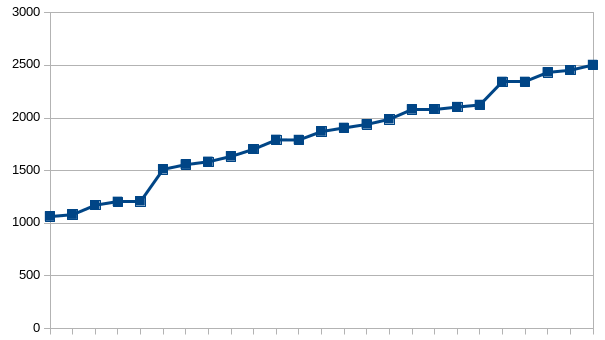
\includegraphics[scale=0.32]{imagens/evolution-s18.png}
    \texttt{s18}
  \end{minipage}
  \begin{minipage}{0.32\textwidth}
    \centering
    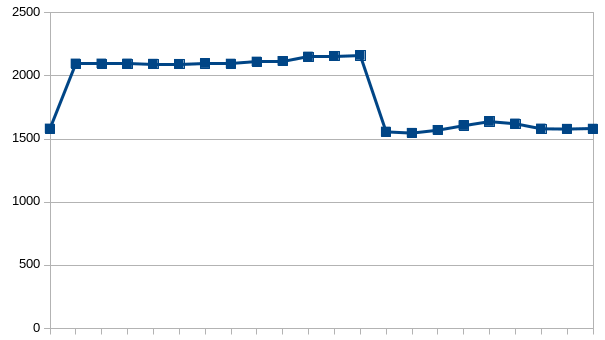
\includegraphics[scale=0.32]{imagens/evolution-s26.png}
    \texttt{s26}
  \end{minipage}

\vspace{3mm}

  \begin{minipage}{0.32\textwidth}
    \centering
    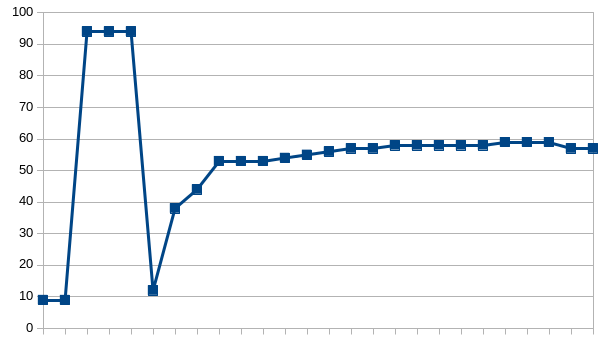
\includegraphics[scale=0.32]{imagens/evolution-s28.png}
    \texttt{s28}
  \end{minipage}
  \begin{minipage}{0.32\textwidth}
    \centering
    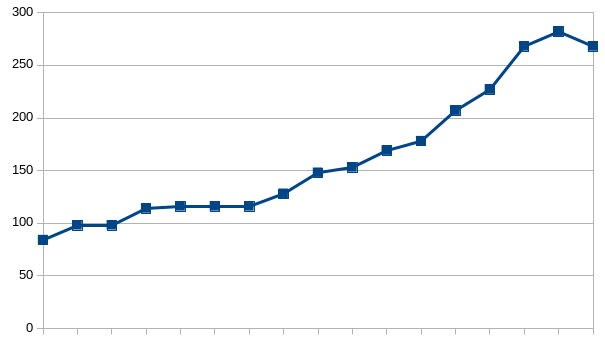
\includegraphics[scale=0.32]{imagens/evolution-s51.png}
    \texttt{s51}
  \end{minipage}
  \begin{minipage}{0.32\textwidth}
    \centering
    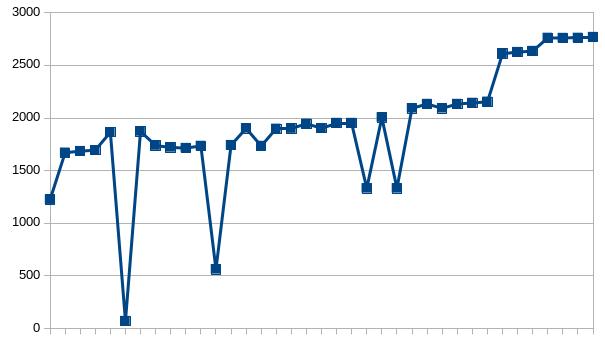
\includegraphics[scale=0.32]{imagens/evolution-s58.png}
    \texttt{s58}
  \end{minipage}
  \caption{Variação no número de módulos dos projetos em fase de {\it Servicing}.}
  \label{evolution-graph}
\end{figure}

% }}}

\section{Ameaças à validade} % {{{

Toda a análise e interpretação dos resultados tomou como base apenas os dados
coletados do site, publicações, e repositórios dos projetos de software
acadêmico de análise estática, o fato de não incluirmos coleta de dados a
partir das pessoas envolvidas nos projetos pode enfraquecer alguma conclusão no
sentido de que alguns projetos podem ter definições explícitas por parte dos
seus desenvolvedores mas que não se refletem ainda nos documentos dos projetos,
apesar disso o nosso estudo tem um caráter exploratório, com interesse especial em
uma figura geral do domínio de análise estática e não necessariamente trazer
evidências sobre os projetos inidivualmente.

% }}}

\section{Conclusões} \label{estudo3:conclusoes} % {{{

Este estudo coletou informações de \ReleasesCount \ lançamentos em relação a
\ProjectsWithReleasesCount \ projetos de software acadêmico de análise
estática. Analisou e extraiu o número de módulos do código fonte de
\ReleasesMetricsCount \ versões distintas destes projetos.

A partir destes dados caracterizou cada um dos \SoftwareCount \ projetos
estudados em relação ao estágio de evolução do ciclo de vida do software e
identificou que a grande maioria encontra-se em estado inicial de
desenvolvimento ou encerrados (76\%).

Apenas 2 projetos encontram-se em evoluçao atualmente, com variação no número
de módulos nos últimos lançamentos recentes superior a 10\%. E 6 projetos em
fase de serviço, indicando que são projetos estáveis com atualizações
constantes mas com pouca variação na base de código do projeto.

Os dados, interpretações e conclusões deste estudo e dos dois estudos
anteriores apresentados nos Capítulos \ref{estudo1} e \ref{estudo2} serão
analisados em conjunto e discutidos no Capítulo seguinte sob uma mesma
perspectiva em relaçao a sustentabilidade técnica do ecossistema de software
acadêmico de análise estática, no recorte de projetos selecionados nas
conferências de Engenharia de Software ASE e SCAM, entre menções encontradas
nas bases ACM e IEEE, e com análise ao nível de código fonte dos projetos
escritos em C, C++ e Java.

% }}}
